\section{Local Asymmetry in the Dalitz Plane}
\label{sec:dalitz}
\label{app:ext_dalitz}
\label{sec:bayes_dalitz}
\emph{In short: the asymmetry is not uniform over the Dalitz plane ($\chi^2=80.8$ for $31$ degrees of freedom); it is concentrated at low $m^2_{\mathrm{lo}}$ outside the $\phi(1020)$ and, in the region of the published analysis of the same data, it reproduces the published value.}
To test whether the asymmetry is uniform over phase space or concentrated in specific regions, each candidate was placed in the Dalitz plane using the two opposite-sign $K^+K^-$ invariant masses $m^2(H1,H2)$ and $m^2(H1,H3)$ (Sec.~\ref{sec:data_presel}), sorted into $m^2_{\mathrm{lo}}$ and $m^2_{\mathrm{hi}}$ to remove the $H2/H3$ labeling ambiguity. The plane $[0,16]\times[0,30]\,\GeV^2$ in $(m^2_{\mathrm{lo}},m^2_{\mathrm{hi}})$ was divided into an $8\times8$ grid, fixed before looking at the asymmetries. In each bin with at least 20 candidates (32 of 64), the local asymmetry $A_i=(N_i^--N_i^+)/N_i$, with binomial uncertainty $\sigma(A_i)=\sqrt{(1-A_i^2)/N_i}$, was compared with the global counting asymmetry $A_{\mathrm{glob}}=-0.043$ through $S_i=(A_i-A_{\mathrm{glob}})/\sigma(A_i)$.

Figure~\ref{fig:bayes_dalitz} shows the occupancy of the bins (a), the local asymmetry (b) and its significance (c). The global homogeneity test, $\chi^2=\sum_iS_i^2=80.8$ for 31 degrees of freedom, holds in the signal window alone ($\chi^2=95.6/28$, signal purity $\approx$96\%), with the $D^0$ veto ($79.2/31$) and with all three charm vetoes ($74.4/31$), and for $6\times6$, $10\times10$ and $12\times12$ grids ($81.0/19$, $97.1/43$, $120.0/60$).

\begin{figure*}[t]
\centering
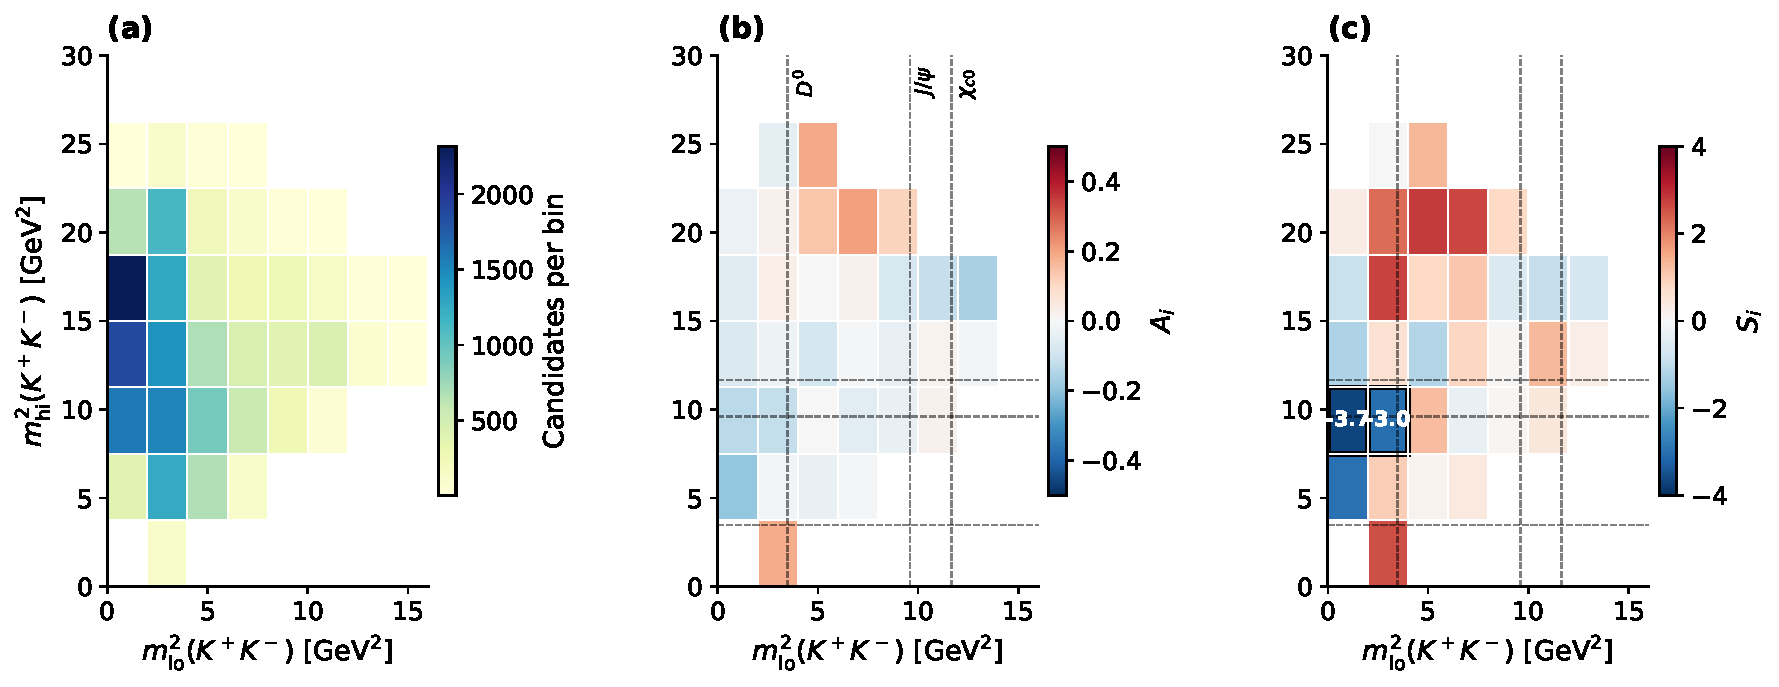
\includegraphics[width=0.95\textwidth]{figures/short_dalitz_maps.pdf}
\caption{Fixed $8\times8$ Dalitz-plot binning, all candidates in the fit window: (a) number of candidates per bin, (b) local asymmetry $A_i$ for bins with $\geq20$ candidates, and (c) local significance with respect to the global asymmetry, $(A_i-A_{\mathrm{glob}})/\sigma(A_i)$. The two bins with $|S_i|>3$ are outlined. Dashed lines: the squared masses of the $D^0$, $J/\psi$ and $\chi_{c0}$, in either opposite-sign pair.}
\label{fig:bayes_dalitz}
\end{figure*}

The structure does not depend on the magnet polarity either. The left-right part of the detection asymmetry changes sign when the polarity is reversed, so a local asymmetry produced by it would appear with opposite deviations in the two samples. In the region of the two significant bins ($m^2_{\mathrm{lo}}<4\,\GeV^2$, $7.5<m^2_{\mathrm{hi}}<11.25\,\GeV^2$) the counting asymmetry is $-0.129\pm0.023$ with the magnet down and $-0.126\pm0.028$ with the magnet up, although the global asymmetries of the two samples differ ($-0.051$ and $-0.032$), and the two maps agree bin by bin ($\chi^2=23.0$ for 29 bins, $p=0.78$). This split does not test the part of the detection asymmetry that does not change sign with the polarity, the different interaction of $K^+$ and $K^-$ with the detector material.
\subsection{Null Tests of the Local-Asymmetry Procedure}
\label{sec:dalitz_null}
\emph{In short: permuting the charges gives $\chi^2=31.5\pm8.4$, as expected, and never reaches the observed $80.8$; the phase-space simulation is consistent with no asymmetry, with slightly optimistic $\chi^2$ $p$-values.}
Two null tests check the procedure itself. Shuffling the charges among the candidates removes any local asymmetry while keeping the occupancy of the bins and the global asymmetry of the data: over $2000$ permutations the $8\times8$ grid gives $\chi^2=31.5\pm8.4$, as expected for 31 degrees of freedom, and no permutation reaches the observed value (permutation $p<5\times10^{-4}$; $p=1\times10^{-3}$ for the $12\times12$ grid). The phase-space simulation of the record, without asymmetry by construction, gives $\chi^2=40.0/30$ ($p=0.11$) with the same procedure on the whole sample; on $500$ subsamples of the size of the data the mean $\chi^2/\mathrm{ndof}$ is $1.16$ and $13\%$ have $p<0.05$, so the $\chi^2$ $p$-values are slightly optimistic (the binomial uncertainty is evaluated at the observed $A_i$). The permutation test, whose null distribution is exact, gives the same conclusion: the non-uniformity is a property of the data.
\subsection{Distribution of the Homogeneity Statistic under Charge Permutation}
\label{app:dalitz_perm}
\emph{In short: shuffling the charges reproduces the $\chi^2$ distribution of a uniform asymmetry, and the observed value lies far beyond all $2000$ permutations.}
For each of $2000$ random permutations of the charges among the candidates, which removes any local asymmetry while keeping the occupancy of the bins and the global asymmetry, the statistic $\chi^2=\sum_iS_i^2$ was computed on the $8\times8$ grid (Fig.~\ref{fig:dalitz_perm}). The distribution follows the $\chi^2$ with $31$ degrees of freedom, which confirms that the statistic is correctly normalized, and no permutation reaches the observed value ($80.8$).

\begin{figure}[t]
\centering
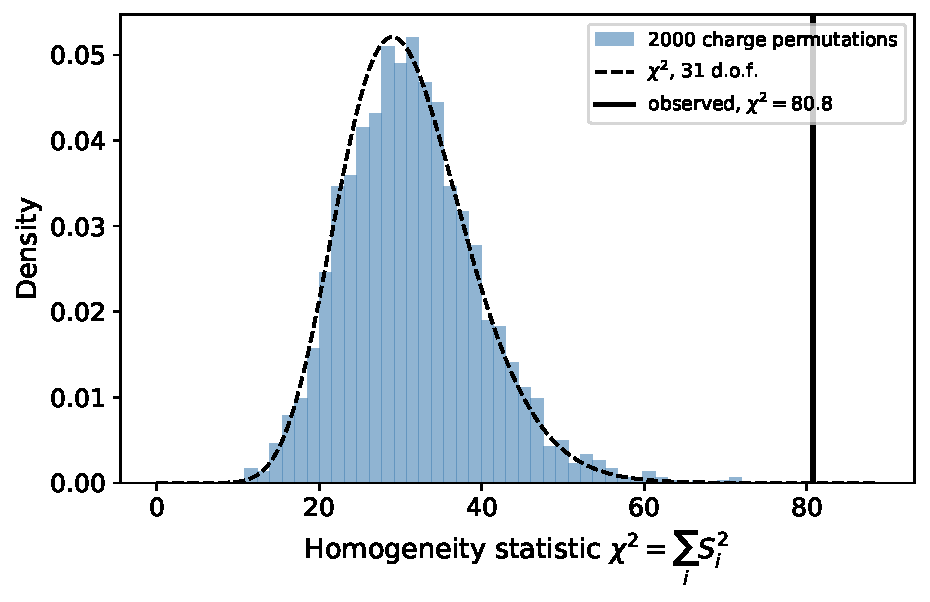
\includegraphics[width=\columnwidth]{figures/dalitz_permutation.pdf}
\caption{Homogeneity statistic $\chi^2=\sum_iS_i^2$ of the $8\times8$ Dalitz grid for $2000$ random permutations of the charges (histogram), $\chi^2$ distribution with $31$ degrees of freedom (dashed) and observed value (line).}
\label{fig:dalitz_perm}
\end{figure}

\subsection{Asymmetry in the $\phi(1020)$ Band and in the Significant Bins}
\label{app:dalitz_phi}
\emph{In short: the band of the $\phi(1020)$ has no asymmetry; the negative asymmetry is outside it, and larger when the $\phi$ candidates are removed.}
The asymmetry is not produced by the $\phi(1020)$ (Fig.~\ref{fig:dalitz_phi}). The band $|m_{\mathrm{lo}}-m_\phi|<10\,\MeV$ around the mass of the $\phi$ (panel~a) contains $1964$ candidates and has a counting asymmetry compatible with zero, $-0.004\pm0.023$, while the region of the two significant bins has $-0.128\pm0.018$ and, without the candidates of the $\phi$ band, $-0.145\pm0.019$; the $353$ candidates of the $\phi$ band that lie in that region have $+0.003\pm0.053$. The region just below the $\phi$ ($m^2_{\mathrm{lo}}<2\,\GeV^2$, outside the band) has $-0.120\pm0.014$ (panel~b).

\begin{figure*}[!t]
\centering
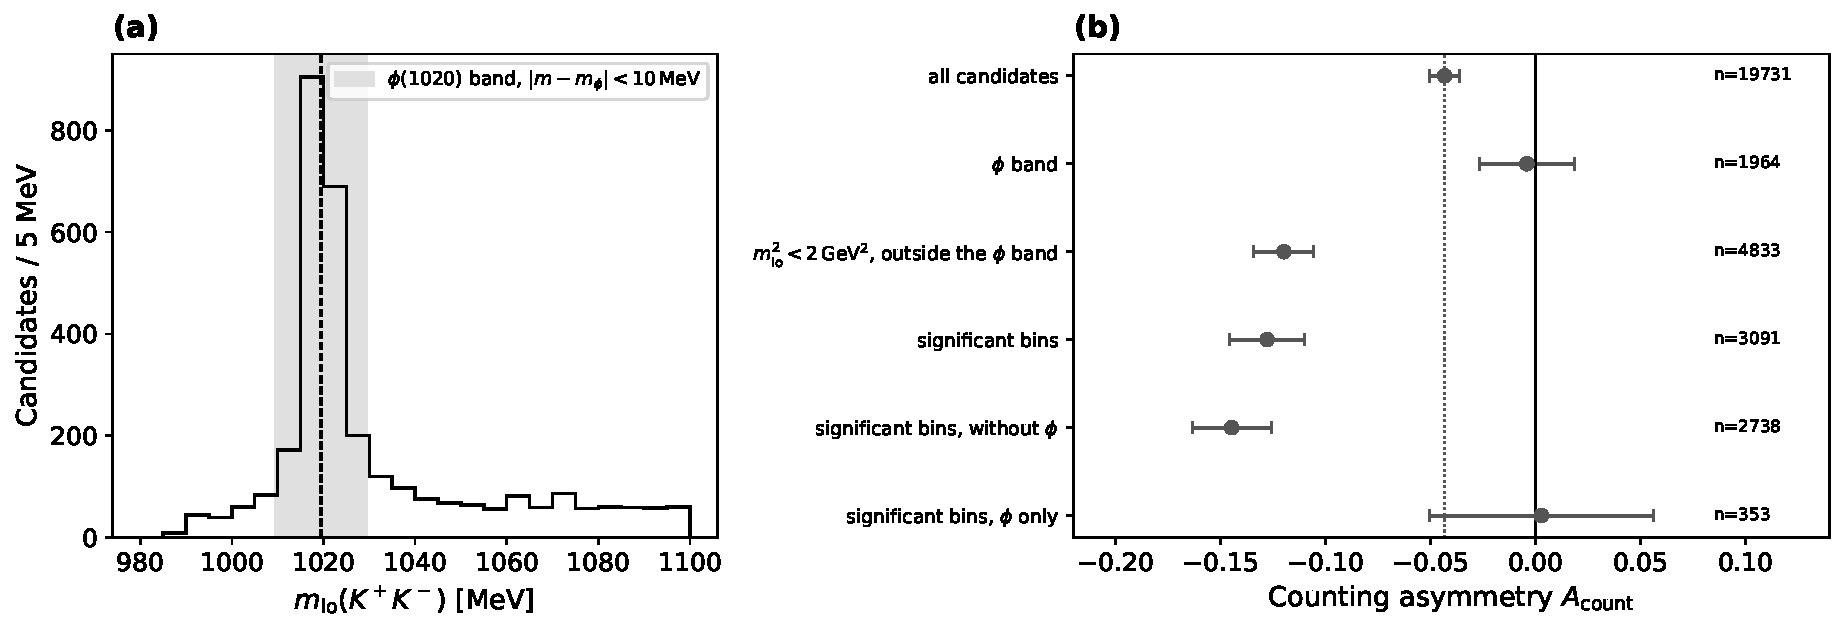
\includegraphics[width=0.9\textwidth]{figures/dalitz_phi_band.pdf}
\caption{(a) Distribution of $m_{\mathrm{lo}}(K^+K^-)$ around the $\phi(1020)$ ($5\,\MeV$ bins) and band used (shaded). (b) Counting asymmetry, with binomial uncertainty and number of candidates, of all candidates (dotted line), of the $\phi$ band, of the region $m^2_{\mathrm{lo}}<2\,\GeV^2$ outside the band, and of the two significant bins of Fig.~\ref{fig:bayes_dalitz}, with and without the candidates of the $\phi$ band, and of those candidates alone.}
\label{fig:dalitz_phi}
\end{figure*}

